\documentclass[a4paper,12pt]{article}

\usepackage[english]{babel}
\usepackage{graphicx}
\usepackage[utf8]{inputenc}
\usepackage{hyperref}

\hypersetup{
  pdftitle={Software developer coffee consumption},
  pdfauthor={Kimmo Puputti},
  pdfsubject={},
  pdfkeywords={},
  pdfcreator={pdflatex},
  pdfproducer={pdflatex},
  colorlinks=true,
  linkcolor=blue,
  citecolor=green,
  filecolor=magenta,
  urlcolor=blue
}


\title{Software developer coffee consumption}
\author{\textbf{Kimmo Puputti}\\kimmo.puputti@futurice.com\\\url{http://kpuputti.fi/}}

\begin{document}

\maketitle
\clearpage

% Introduction
\section{Introduction}

There is a famous quote by Alfréd
Rényi\footnote{\url{http://en.wikipedia.org/wiki/Alfr\%C3\%A9d_R\%C3\%A9nyi}}
about mathematicians:\\

\textit{``A mathematician is a device for turning coffee into theorems.''}\\

\noindent This quote has been widely applied to programmers as well in
the form:\\

\textit{``A programmer is a device for turning coffee into code.''}\\

\noindent There has also been active discussion in the
web\footnote{\url{http://giorgiosironi.blogspot.com/2010/03/coffee-and-programming.html}} \footnote{\url{http://programmers.stackexchange.com/questions/107142/is-there-something-special-about-coffee-and-programming}}
about the coffee drinking habits of programmers. But is there any
scientific validation of this popular myth? The goal of this work is
to take a representative sample of programmers and analyze their
(coffee) drinking habits.

% Research Question
\section{Research Question}
\label{rq}

The objective of this work is to answer the following questions:

\begin{itemize}
\item Do programmers drink coffee on daily basis?
\item How much coffee do programmers drink on daily basis?
\end{itemize}

% Methods
\section{Methods}
\label{methods}

The research question posed in Section \ref{rq} was answered by making
a face-to-face user survey (see Appendix \ref{survey}). The survey was
presented to programmers in the Futurice office.

% Results
\section{Results}

The results presented in Appendix \ref{survey} and visualized in
Appendix \ref{charts} show that approximately 73 \% of the developers
surveyed drink coffee with an average of 3.2 cups a day.

% Discussion
\section{Discussion}

% Problems:
% - What numbers are the results compared to?
% - How big is a cup?
% - What if people drink several different drinks?
% - Is Futurice employees representative of the Software Developer community?
% - Is the surveyed sample representative of Futurice employees?

In this paper the myth of programmers being avid coffee drinkers was
validated. The representative sample was taken in Futurice offices. It
was noticed that a large portion of the surveyed developers do drink
coffee and several cups per day, but there is no other data to compare
with.

Also, it is open to discussion whether the sample truly represents the
software developer community because Futurice employees are younger
than the average developers in the industry.

Some future improvements were considered to the research methods
defined in Section \ref{methods}:

\begin{itemize}
\item What is the definition of a cup?
\item What if people drink different kinds of drinks on daily basis?
\end{itemize}

\noindent We leave these improvements for future research.

\clearpage
\appendix
\section{Survey Questionnaire and Answers}
\label{survey}

On average, what and how many cups do you drink on daily basis?\\

\begin{tabular}{|r|l|l|}
  \hline
  \textbf{subject} & \textbf{What?} & \textbf{How many cups?} \\
  \hline
  1 & coffee & 2-3 \\
  2 & tea & 7 \\
  3 & coffee & 1 \\
  4 & coffee & 3-4 \\
  5 & coffee & 5-8 \\
  6 & coffee & 3-5 \\
  7 & battery & 1 \\
  8 & coffee & 2-4 \\
  9 & tea & 12-14 \\
  10 & sparkly water & 5-6 \\
  11 & coffee & 6 \\
  12 & coffee & 3-4 \\
  13 & coffee & 3 \\
  14 & coffee & 0-1 \\
  15 & coffee & 2 \\
  \hline
\end{tabular}

\clearpage
\section{Charts}
\label{charts}

\begin{figure}[h]
  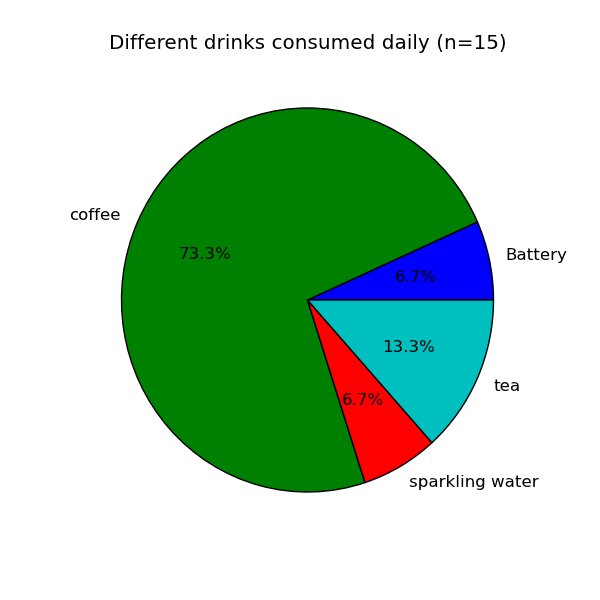
\includegraphics[width=\textwidth]{drinks.png}
\end{figure}

\begin{figure}[h]
  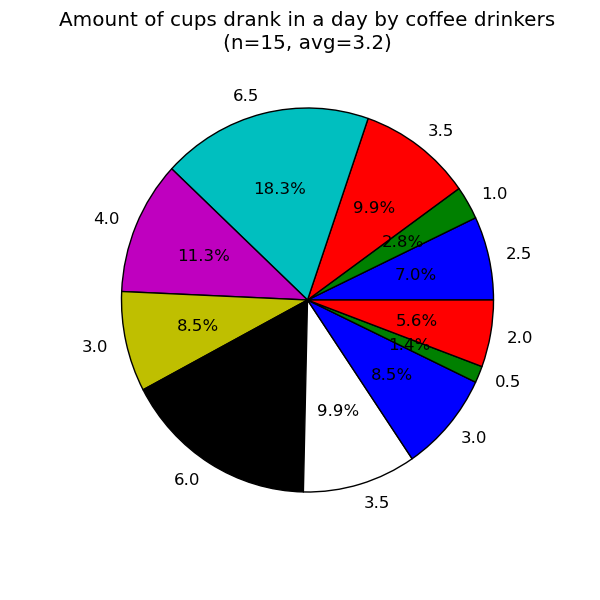
\includegraphics[width=\textwidth]{amounts.png}
\end{figure}

\end{document}
